\part{Tutoriel}
\chap{Votre premier projet de robotique}\label{ch.intro}

\sect{Faire connaissance avec Thymio}

La \cref{fig.front} montre l'avant et le dessus de Thymio.
Vous pouvez voir le bouton central rond (\textcolor{blue}{A}), entouré de quatre boutons triangulaires (\textcolor{blue}{B}).
Ce sont des boutons tactiles, un simple effleurement suffit à les activer.
Juste derrière ces boutons se trouve un indicateur en forme de pile (\textcolor{blue}{C}).
Une, deux ou trois petites barres de lumière verte affichent l'état de charge du robot.
Sur l'arrière du robot, nous voyons les lumières du haut (\textcolor{blue}{D}), allumées en rouge sur cette photo.
Il y a des lumières similaires sur le bas du robot (voir \cref{fig.bottom}).
Enfin, les petits rectangles noirs à l'avant du robot (\textcolor{blue}{E}) sont des capteurs infrarouge de distance, vous en saurez plus dans le \cref{ch.pet}.

\begin{figure}[h]
\begin{center}
\gr{front}{.8}
\caption{L'avant et le dessus de Thymio}\label{fig.front}
\end{center}
\end{figure} 

\sect{Connecter le robot, démarrer Aseba et lancer VPL}

Pour commencer, connectez Thymio à votre ordinateur à l'aide du câble USB fourni avec le robot.
Si la connection est réussie, le robot jouera quelques notes.
S'il est éteint, touchez simplement son bouton central pendant quelques secondes jusqu'à entendre quelques notes.
Lancez VPL en double-cliquant sur l'icône \blksm{thymiovpl} de votre ordinateur.

\importantbox[Petites images]{
Quand le texte contient une petite image, la même image en plus grand apparaît aussi dans la marge.}


Il se peut que VPL se connecte directement à votre robot.
Si ce n'est pas le cas, la fenêtre montrée dans la \cref{fig.connect} devrait apparaître.
Cochez la case \bu{Port série}, cliquez sur \bu{Thymio-II Robot}, sélectionnez \bu{Français} et cliquez sur \bu{Connecter}.
En fonction de la configuration de votre ordinateur et de votre système d'exploitation, il peut y avoir plusieurs entrées dans la liste des ports séries et le texte à côté de \bu{Thymio-II Robot} peut différer de la \cref{fig.connect}.

\trickbox{Il est aussi possible d'accéder à VPL depuis Aseba Studio, l'environement de programmation textuelle, à travers le \textit{plugin} VPL qui se trouve dans la zone \textit{Outils} en bas à gauche de l'écran.}

\begin{figure}
\begin{center}
\gr{connect}{.4}
\caption{Se connecter à Thymio via le port série (USB)}\label{fig.connect}
\end{center}
\end{figure}

\newpage

\sect{L'interface VPL}

L'interface VPL est illustrée ci-dessous.
Elle est composée de six zones :
\begin{enumerate}[noitemsep,nosep]
\item Une barre d'outils avec les boutons pour créer un nouveau programme, en ouvrir un existant, sauvegarder, lancer le programme, etc.
\item La zone de programmation pour construire le programme qui contrôlera Thymio.
\item Une zone de messages qui donne les messages d'erreur lorsque le programme n'est pas construit correctement.
\item Les blocs d'événement disponibles pour construire votre programme.
\item Les blocs d'action disponibles pour construire votre programme.
\item La traduction du programme en AESL, le langage textuel d'Aseba.
\end{enumerate}

\plainfloat
\begin{figure}[h]
\gr{gui}{1}
\caption{La fenêtre de VPL}\label{fig.vplgui}
\end{figure}
\framedfloat

\bigskip

\informationbox{Pour aller plus loin}{
Dès que vous créez un programme en utilisant VPL,
la traduction du programme dans le langage de programmation textuel AESL apparaît dans la partie droite de la fenêtre.
C'est en fait ce code AESL qui est interprêté par le robot.
Si vous êtez curieux et que vous désirez comprendre ce langage, vous pouvez lire le \cref{ch.next} qui explique ces traductions.
Vous pouvez ensuite vous rendre sur \href{https://aseba.wikidot.com/fr:asebausermanual}{https://aseba.wikidot.com/fr:asebausermanual} 
pour les références et en apprendre plus sur AESL et son environnement Studio.}

\newpage

\sect{Écrire un programme}

Quand vous démarrez VPL, une zone de programmation vide est affichée.

Si, après avoir construit un bout de programme, vous voulez effacer le contenu de la zone de programmation, vous pouvez cliquer sur \blksm{new} (\bu{Nouveau}).

Un programme dans VPL consiste en des \emph{paires événement-actions}, chacune construite en mettant ensemble un bloc événement et un ou plusieurs bloc action.
Par exemple, la paire : \blkc{e-a-pair} allume la lumière du haut du Thymio en rouge lorsque l'on touche le bouton avant sur le robot.

\importantbox[Signification d'une paire événement-actions]
{
\centering
Lorsque l'événement se produit, le robot exécute les actions associées.}

Dans la zone de programmation se trouve initialement une paire événement-actions vide: \blkc{empty-frame}
Pour placer un bloc dans le programme depuis une des colonnes (zones 4 et 5 de \cref{fig.vplgui}), cliquez puis gardez enfoncé le bouton gauche de la souris.
Glissez ensuite le bloc jusqu'à un carré traitillé.
Lorsque le bloc est au-dessus du carré, relâchez le bouton de la souris pour déposer le bloc à sa place.

\importantbox{
On appelle \emph{glisser-déposer} (ou \emph{drag-and-drop} en anglais) la technique qui vient d'être décrite.
Elle est fréquemment utilisée dans les interfaces de programmes.}

Commencez par amener le bloc évenement boutons \blksm{event-buttons} sur le carré vide de gauche.
Vous recevrez alors un message vous invitant à ajouter un bloc action.
Amenez le bloc action couleur du haut \blksm{action-colors-up} sur le carré de droite.
Et voilà ! Vous avez construit une paire événement-actions !

Il nous faut maintenant modifier l'événement et l'action pour qu'ils fassent ce que l'on veut.
Pour l'événement, cliquez sur le bouton avant (le triangle supérieur) ; il va devenir rouge : \blkc{forward}
Cela signifie qu'un événement se produira lorsque le bouton \emph{avant} de Thymio sera touché.

Le bloc action couleur contient trois \textit{sliders} --- des barres de couleur avec un carré blanc.
Chaque barre règle une des trois couleurs primaires rouge, vert et bleu.
Si vous déplacez un de ces carrés blanc vers la droite et revenez ensuite en arrière,
vous vous apercevrez que le fond du bloc change de couleur.
En mélangeant ces trois couleurs primaires (rouge, vert et bleu),
toutes les couleurs peuvent être créées.
Déplacez le \textit{slider} rouge jusqu'à ce que le carré soit
tout à droite et déplacez les \textit{sliders} vert et bleu tout à gauche.
La couleur sera toute rouge sans composante bleu ou vert : \blkc{red}

\sect{Sauvegarder le programme}

Avant de lancer votre programme, sauvegardez-le sur votre ordinateur.
Cliquez sur l'icône \blksm{save} (\bu{Sauvegarder}) de la barre d'outils.
Vous devrez choisir un nom pour votre programme, par exemple \bu{afficher-rouge}.
Choisissez l'endroit où vous voulez sauvegarder le programme, sur le bureau par exemple, et cliquez sur \bu{Sauvegarder}.

\importantbox[Sauvegardes fréquentes]{
Lorsque vous modifiez un programme,
cliquez souvent le bouton \bu{Sauvegarder} pour éviter de 
ne perdre votre travail si un problème devait survenir avec votre ordinateur.}

\sect{Lancer le programme}

Pour lancer le programme, cliquez sur \blksm{run} (\bu{Lancer}) dans la barre d'outils.
Essayez maintenant d'appuyer sur le bouton avant de Thymio, il devrait s'être allumer en rouge!

\informationbox{Félicitations !}{
Vous avez créé et exécuté votre premier programme.
Voici ce qu'il fait :\\
\textbf{Lorsque l'on touche le bouton avant de Thymio, il devient rouge.}}

Si vous voulez arrêter le programme VPL, cliquez sur \blksm{stop} (\bu{Stop}).
Ceci peut être très utile lorsque par exemple vous exécutez un programme qui fait avancer le robot mais que vous avez oublié d'ajouter une paire événement-actions pour arrêter les moteurs.

\sect{Éteindre le robot}

Lorsque vous avez terminé d'utiliser Thymio, vous pouvez l'éteindre en touchant son bouton central et en gardant le contact quelques secondes.
Vous entendrez quelques notes et Thymio s'arrêtera.
Tant que le robot est connecté à un ordinateur, sa batterie continue à se recharger. Une petite lumière rouge à l'arrière du robot, juste à côté du câble USB, permet de savoir s'il est rechargé ou pas. La lumière passe du rouge au bleu pour indiquer qu'il est complètement rechargé, comme sur la \cref{fig.back}.
Vous pouvez déconnecter le cable quand vous n'utilisez pas le robot.

\trickbox{
Si vous voulez charger le robot plus vite, vous pouvez le connecter à une prise murale avec un chargeur pour téléphone portable fournissant une prise micro-USB.
}

\begin{figure}
\begin{center}
\gr{back}{.6}
\caption{L'arrière de Thymio avec le câble microUSB et le témoin de charge}\label{fig.back}
\end{center}
\end{figure}

Si le cable USB se déconnecte durant la programmation, VPL attendra une reconnection.
Vérifiez les deux côtés du cable, débranchez et rebranchez le câble, et regarder si VPL fonctionne.
Si vous avez un problème, vous pouvez toujours fermer VPL, reconnecter le robot et réouvrir VPL.

\sect{Modifier un programme}

\begin{itemize}
\item Pour effacer une paire événement-actions, cliquez sur \blksm{x}, en haut à droite de la paire.
\item Pour ajouter une paire événement-actions, cliquez sur \blksm{plus}, disponible en dessous de chaque paire.
\item Pour déplacer une paire événement-actions, maintenez le bouton gauche de la souris enfoncé sur une paire et glissez la à l'endroit désiré.
\item Pour copier une paire événement-actions vers un deuxième endroit dans le programme, appuyez et maintenez pressé la touche \bu{Ctrl} et utilisez votre souris pour glisser et déposer la paire à l'emplacement désiré.\label{p.copy-pairs}\footnote{Sur Mac OS, la touche \bu{Command} remplace la touche \bu{Ctrl}.}
\end{itemize}

\informationbox{Le bouton \bu{Lancer} clignote}{
Lorsque vous modifiez un programme, le bouton \bu{Lancer} clignote en bleu et vert pour vous rappeler qu'il faut cliquer sur le bouton pour charger le programme modifié vers le Thymio.\label{p.blink}}

Si vous voulez tester une modification sans perdre votre programme actuel, vous pouvez créer une copie du programme actuel en cliquant sur \blksm{saveas} (\bu{Sauvegarder sous}) et en entrant un nouveau nom de fichier.

\sect{Ouvrir un programme existant}

Si vous voulez continuer un programme que vous aviez commencé précédemment, il suffit de l'ouvrir avec l'interface VPL pour le modifier ou l'améliorer.
Cliquez sur l'icône \blksm{open} (\bu{Ouvrir}) et sélectionnez le fichier que vous voulez ouvrir, par exemple \bu{afficher-rouge}.
Les paires événement-actions du programme vont être affichées dans la zone de programmation, et vous pourrez continuer à les modifier.

%\newpage
\sect{La paire événement-actions actuelle}

Lorsque vous cliquez sur une paire événement-actions,
celle-ci s'affiche avec un fond jaune.
Il en va de même lorsque vous ajoutez un bloc événement ou action dans une paire vide.

\begin{center}
\begin{tabular}{c@{\hspace{.1\textwidth}}c}
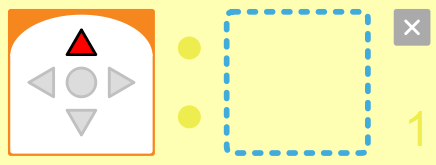
\includegraphics[width=.3\textwidth,keepaspectratio=true]{event-action-pair-yellow1}
&
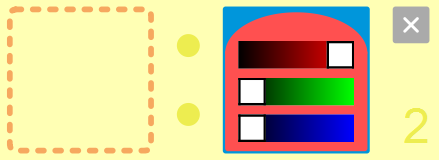
\includegraphics[width=.3\textwidth,keepaspectratio=true]{event-action-pair-yellow2}
\end{tabular}
\end{center}

Le carré gauche de couleur dorée est l'espace réservé à l'événement;
le carré bleu à droite sert d'emplacement à la première (ou unique) action.
La pair au fond jaune est appelée la paire actuelle.

\informationbox{Insérer un bloc rapidement}{
Si vous cliquez sur un bloc événement ou action,
il sera automatiquement placé dans la zone de programmation dans la paire événement-actions sélectionnée.}

\bigskip\bigskip

\informationbox{La barre d'outils VPL}{
L'\cref{a.toolbar} contient une description de tous les boutons
de la barre d'outils VPL.
Consultez la de temps en temps jusqu'à ce que vous ayez appris à les utiliser.}
